%==============================================================================
% Sjabloon poster bachproef
%==============================================================================
% Gebaseerd op document class `a0poster' door Gerlinde Kettl en Matthias Weiser
% Aangepast voor gebruik aan HOGENT door Jens Buysse en Bert Van Vreckem

\documentclass[a0,portrait]{hogent-poster}

% Info over de opleiding
\course{Bachelorproef}
\studyprogramme{toegepaste informatica}
\academicyear{2024-2025}
\institution{Hogeschool Gent, Valentin Vaerwyckweg 1, 9000 Gent}

% Info over de bachelorproef
\title{Hoe kan trust management effectief worden geïmplementeerd voor het beveiligen van bedrijven met heterogene gesegmenteerde netwerken?}
%\subtitle{Ondertitel (eventueel)}
\author{Thibo Haezaert}
\email{thibo.haezaert@student.hogent.be}
\supervisor{Gilles Blondeel}
\cosupervisor{Dirk Mussen (KBC)}

% Indien ingevuld, wordt deze informatie toegevoegd aan het einde van de
% abstract. Zet in commentaar als je dit niet wilt.
\specialisation{Systeem- en Netwerkbeheer}
\keywords{Root certificates, Truststores, Trust management, SCCM, Chef, Ansible, HashiCorp Vault}
%\projectrepo{https://github.com/user/repo}

\begin{document}

\maketitle

\begin{abstract}
In moderne, heterogene bedrijfsnetwerken is het essentieel om zorgvuldig te bepalen welke systemen welke root- en intermediate-certificaten vertrouwen. Dit proces, bekend als trust management, houdt niet alleen het technisch beheren van truststores in, maar vooral het strategisch toewijzen van vertrouwen op basis van de rol, locatie of functie van een systeem binnen het netwerk.

Een foutieve toekenning van vertrouwen kan leiden tot verhoogde cyberrisico’s of het falen van kritieke communicatie. Deze bachelorproef onderzoekt hoe trust management effectief kan worden geïmplementeerd binnen gesegmenteerde netwerken met zowel Windows- als Linux-systemen.

Na een literatuurstudie werd een proof-of-concept uitgewerkt waarin vier beheeroplossingen werden getest:

\begin{itemize}
  \item Windows: via Group Policy Objects (GPO) en System Center Configuration Manager (SCCM)
  \item Linux: via Ansible en Chef
\end{itemize}

Deze tools maken het mogelijk om truststores centraal te beheren en contextspecifiek toe te wijzen, afgestemd op netwerksegmentatie.

Aanbevelingen richten zich op integratie met bestaande PKI-processen, uitbreidbaarheid naar grotere infrastructuren en verfijnde toewijzingscriteria.

Onderwerpen zoals security, MacOS en IoT vielen buiten scope en vormen mogelijkheden voor toekomstig onderzoek.
\end{abstract}

\begin{multicols}{2} % This is how many columns your poster will be broken into, a portrait poster is generally split into 2 columns

\section{Introductie}

Moderne bedrijfsnetwerken zijn vaak \textit{heterogeen} en \textit{gesegmenteerd}, wat het beheer van vertrouwensrelaties tussen systemen bemoeilijkt. Een cruciaal onderdeel hiervan is het bepalen welke root- en intermediate-certificaten elk systeem mag vertrouwen.

\textit{Trust management} verwijst naar het centrale proces waarbij organisaties certificaatvertrouwen toewijzen aan systemen op basis van hun rol, locatie of functie binnen het netwerk. Onvoldoende of overmatig vertrouwen in certificaten verhoogt respectievelijk het risico op operationele fouten of beveiligingsincidenten.

Deze bachelorproef onderzoekt hoe trust management effectief kan worden geïmplementeerd in zulke netwerken. De focus ligt op:

\begin{itemize}
    \item Tools en technieken voor truststorebeheer en hun beperkingen.
    \item Centraal beheer van truststores over diverse endpoints.
    \item Differentiatie per netwerksegment.
    \item Implementatie in een proof-of-concept omgeving.
    \item Evaluatie van effectiviteit en schaalbaarheid.
    \item Praktische aanbevelingen voor bedrijven.
\end{itemize}


\section{Proof-of-concept}

Een virtuele proof-of-concept omgeving werd opgezet met Windows- en Linux-endpoints, verdeeld over gesegmenteerde netwerken. Elk segment kreeg een eigen set root-certificaten toegewezen.

In de eerste oplossing werd gebruikgemaakt van \textbf{GPO’s} (Windows) en \textbf{Ansible} (Linux) om certificaten toe te wijzen op basis van OU’s of end-point groepering. Deze methode bleek echter beperkt in schaalbaarheid: PowerShell ondersteunt geen beheer van GPO-certificaten, en Ansible vereist SSH-connecties naar alle endpoints.

\begin{center}
  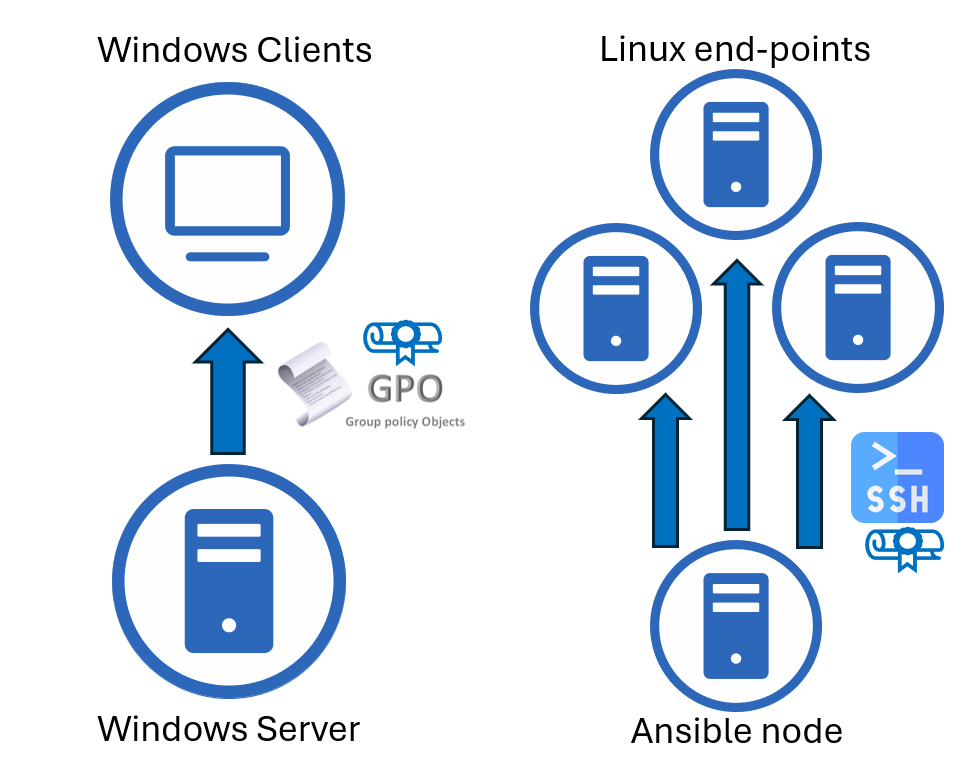
\includegraphics[width=0.5\linewidth]{Process_opl1}
  \captionof{figure}{Procesoverzicht oplossing 1}
\end{center}

De tweede oplossing verbeterde de schaalbaarheid door gebruik te maken van \textbf{SCCM} met PowerShell-scripts (Windows) en \textbf{Chef} cookbooks (Linux). Beide platformen haalden certificaten op uit een centrale \textbf{HashiCorp Vault}, gestructureerd per netwerksegment. Endpoints selecteerden de juiste segmentdata via parameters of node-attributen.

\begin{center}
  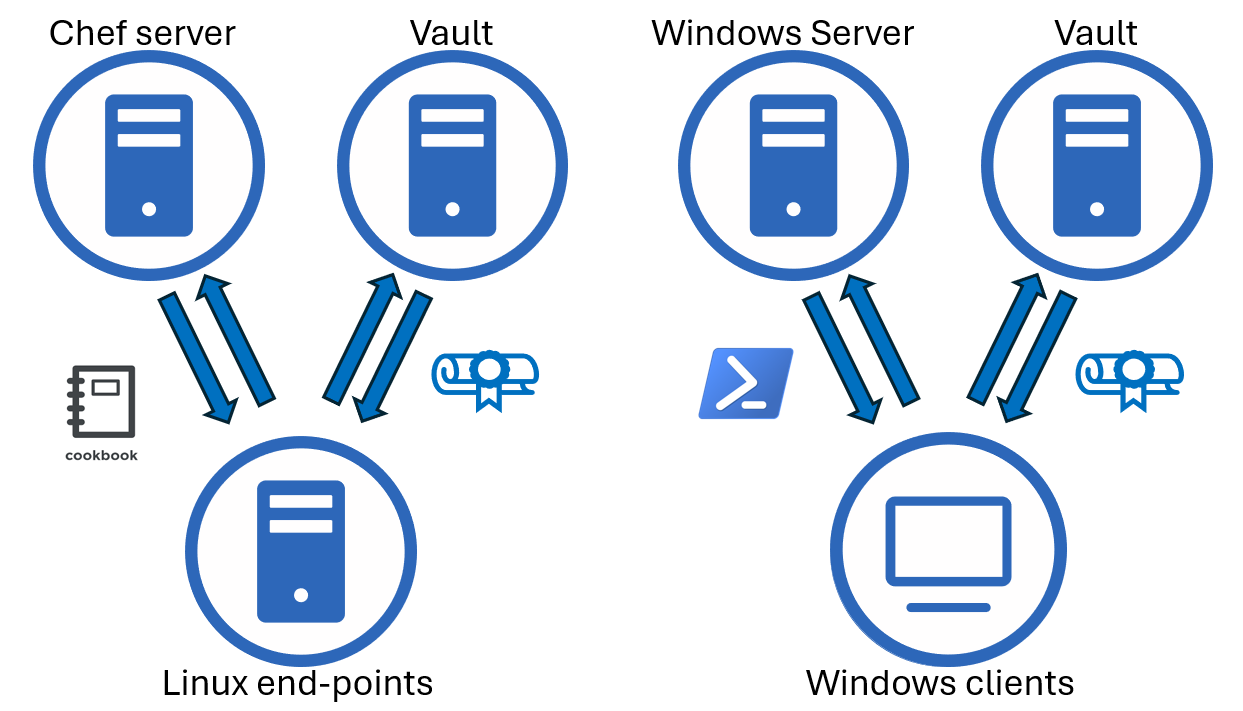
\includegraphics[width=0.5\linewidth]{Process_opl2}
  \captionof{figure}{Procesoverzicht oplossing 2}
\end{center}

\section{Conclusies}

Dit onderzoek toont aan dat trust management effectief geïmplementeerd kan worden via een gecentraliseerde architectuur waarin de inhoud van truststores per systeem verschilt op basis van netwerksegmentatie.

De combinatie van een centrale certificaatbron (zoals HashiCorp Vault) met tools zoals GPO’s, SCCM (Windows) en Ansible of Chef (Linux) maakt het mogelijk om root- en intermediate-certificaten doelgericht te verdelen.

Elke oplossing heeft voor- en nadelen in termen van schaalbaarheid, snelheid en beheercomplexiteit. De proof-of-concept bevestigt dat organisaties trust kunnen toewijzen op basis van een andere gewenste context (bv. segment, rol, locatie), zolang de onderliggende tooling hierop wordt afgestemd.

\section{Toekomstig onderzoeken}

Hoewel de voorgestelde oplossing succesvol werd gevalideerd in een gecontroleerde proof-of-concept omgeving, blijven er verschillende pistes voor verder onderzoek. Enkele belangrijke aandachtspunten zijn:

\begin{itemize}
    \item \textbf{Schaalbaarheid}: Onderzoeken hoe de architectuur presteert in grootschalige productienetwerken met honderden tot duizenden endpoints.
    
    \item \textbf{Integratie met PKI}: Analyseren hoe truststore-updates kunnen worden afgestemd op certificaatlevenscycli via bestaande Public Key Infrastructure (PKI)-diensten.
    
    \item \textbf{Ondersteuning van andere platformen}:
    \begin{itemize}
        \item \textit{macOS}: Verkennen van beheermogelijkheden voor Apple-systemen.
        \item \textit{IoT-apparaten}: Aangepaste methoden ontwikkelen voor devices die niet ondersteund worden door klassieke tools.
    \end{itemize}
    
    \item \textbf{Beveiligingsanalyse}:
    \begin{itemize}
        \item Beveiligen van de centrale certificaatbron (bijv. HashiCorp Vault).
        \item Garanderen van integriteit en authenticiteit van communicatie tussen beheertools en endpoints.
    \end{itemize}
\end{itemize}

\end{multicols}
\end{document}